\section{Rare, radiative and semileptonic $B$ decays}

Rare decays of $B$ mesons are natural candidates to be studied within the indirect approach: being dominated by  loop and box diagrams, they are very suppressed in the SM, and so the most sensitive to variations due to NP.  
Among them, radiative $B$ decays, with the emission of a virtual or real photon, as well as semileptonic $B$ decays are extremely interesting, as the theory has the instruments to perform very precise predictions.  A joint work between experimentalists and theorists has allowed to identify an ensemble of observables which are
at the same time sensitive to the couplings to different possible sources of NP and as immune as possible to non factorizable QCD effects. 
With the abundance of data produced by the LHC collisions, for the first time some of these decays can be observed, their properties measured  and the prediction tested with better precision than ever.  The French community is largely active both on the experimental and theoretical side on rare, radiative and semileptonic decays.  In the need of exchanging results, it has been promoting in the past years the aforementioned PEPS-PTI projects and the related workshops, successfully followed by the community. 


The LHCb collaboration has produced a large set of results, related to the exclusive $b \to s\ell \ell $ decay modes, which  are currently dominating the field.  
In the special case of the $\cb(B_s\to \mu\mu)$, the CMS collaboration is also significantly contributing and after combining the results of the two experiments, 
it turned out that the long searched $\cb(B_s\to \mu\mu)$ is only slightly lower than, but compatible with, the value
predicted in the SM~\cite{CMS:2014xfa}. The $B_d\to \mu\mu$ decay has also been seen, its branching ratio turning out to be compatible with the value predicted by the SM. 
\par
On the other hand,  after comparing the experimental values of $B\to K^\ast \mu\mu$  angular observables~\cite{Aaij:2015oid}, as well as of $\cb(B\to K \mu\mu)$~\cite{Aaij:2014pli} and $\cb(B_s\to \phi \mu\mu)$~\cite{Aaij:2015esa}, with the theoretical estimates derived in the SM, 
one finds considerable discrepancies, of the order of 3 to 3.5 standard deviations~\cite{Altmannshofer:2015sma, Descotes-Genon:2015uva, Descotes-Genon:2016hem}.  The LHCb results of the $B^0\to K^\ast \mu\mu$  angular analysis were also recently confirmed  by the Belle collaboration~\cite{Abdesselam:2016llu}.  
It appears, however, that the most significant discrepancies occur near the charm production threshold, a region notoriously difficult for the theoretical 
description of these decays. In fact in this region it is required an accurate estimate of the hadronic matrix element of a non-local operator corresponding to disconnected $c\bar c$-diagrams, which 
cannot be computed by means of numerical simulations of QCD on the lattice. For that reason, as of now, it is not clear whether the current discrepancies are due to the lack of theoretical 
control of the $c\bar c$ contributions~\cite{Ciuchini:2015qxb}, or they indicate the presence of NP couplings. If the second option is adopted, the angular observables of $B\to K^\ast \mu\mu$ and $B_s\to \phi \mu\mu$ 
decays  provide very stringent constraints on the scenarios of NP. An example of the current constraint is shown in figure~\ref{figrare} on the left. 

On top of the very rich set of results involving muons, LHCb has also performed an angular analysis  of the $B^0\to K^\ast e e $ decay mode in the low dilepton invariant mass region $q^2$~\cite{Aaij:2015dea}. The results found  are in agreement with SM but currently quite limited in statistics.    With more data coming, the electron channels will be more and more competitive with the muon channels and their measurements more precise. In addition, among other observables, they  provide a  determination of the photon polarization, as the di-electron are emitted by a virtual photon in some part of the kinematic space.  This is a complementary measurement to the one of the decays involving real photons, like $B_s \to \phi \gamma$ and $B\to K^* \gamma$.  In the SM the photon polarization  in $b \to s \gamma$ transition is  known to be left (right) for a $b$ ($\bar b$) quark, modulo effect of the order of $4\%$  due to the quark masses and the emission of soft gluons. Any deviation from this precise expectation would be a clear sign of NP.  In the next years precise measurements of the photon polarization in $b \to s \gamma$ transitions are expected to come, but some challenges need to be faced, like for example the study of the resonant $K^*$ structure, which needs a close collaboration between theorists and experimentalists. 

Another experimental result which has also provoked some interest in the flavor physics community is that the observable $R_K = \cb(B\to K\mu\mu)/\cb(B\to Kee)_{{\rm low}-q^2}$  was found to be $2.6\sigma$ smaller than  predicted in the SM~\cite{Aaij:2014ora}, as shown in figure~\ref{quarklep}, which suggests the violation of the universality of the coupling to leptons (LFUV). This is also hilighted by the phenomenological analysis shown in figure~\ref{figrare} on the right. Such a puzzling phenomenon should be scrutinized with higher statistics and tested in other similar situations, 
for example measuring $R_K$ at high-$q^2$'s, $R_{K^\ast}$, $R_{\Lambda^{(\ast )}}$ at both low- and high-$q^2$. This observation is adding to an already noted problem of $R_{D^{(\ast)}}=  \cb(B\to D^{\ast}\tau\nu_\tau)/\cb(B\to D^{\ast}\mu\nu_\mu)$ for which the experimental result, first measured at the $B$-factories~\cite{Huschle:2015rga} and then confirmed by LHCb~\cite{Aaij:2015yra}, is in between 2 and 4$\sigma$ larger than what is predicted in the SM~\cite{bib:hfag}. There are very few phenomenologically viable theoretical scenarios of NP which can simultaneously explain that $R_K^{\rm exp}<R_K^{\rm SM}$ and that $R_{D^{(\ast )}}^{\rm exp} > R_{D^{(\ast )}}^{\rm SM}$~\cite{Bhattacharya:2014wla}. To further understand the origin of the LFUV one can envisage doing the angular analysis of all the mentioned decay modes, and from the ratios of angular observables check whether or not a similar size of the LFUV is indeed observed. 
Furthermore, to facilitate a comparison with theory it is more sound to compare $B_s\to D_s^{(\ast)}\ell \nu_\ell$ decays, because the theoretical uncertainty related to the chiral extrapolation in the light valence quark on the lattice is completely avoided in this way. Moreover, the emission of soft photons can differently affect $B^- \to D^{0 (\ast)}\ell^- \bar \nu_\ell$ and $B^0 \to D^{- (\ast)}\ell^+ \nu_\ell$, the modes which are usually averaged. Such a problem is much less significant if one works with $B_s\to D_s^{(\ast)}\ell \nu_\ell$ decays. 

Most of the models proposed for describing the LFUV effects hinted at by $R_K$
allow for lepton flavor violation (LFV) too, after the general connection
between LFUV and LFV was emphasized in Ref. \cite{Glashow:2014iga}. Here it
was also shown that the size of the $R_K$ departure from unity alone allows
to estimate the natural size expected for LFV $B$ decays to be of the order 
of $10^{-8}$, which happens to be within LHCb reach at Run2. This conclusion
was corroborated by a number of follow-up studies, e.g.
\cite{Guadagnoli:2015nra,Boucenna:2015raa}. For that reason it is of great interest to measure the LFV modes such as $B_s\to \mu \tau$, $B\to K^{(\ast )}\mu \tau$,  $B_s\to \phi \mu \tau$, which can now be probed thanks to the large statistics achievable at the LHC. The experimental bounds on $\cb(B_s\to \mu e)$ and $\cb(B_s\to K^{(\ast )} \mu e)$ can also be greatly improved. These results can be very useful for phenomenology of the LFV decays and for the bigger picture that could ultimately lead to a theory of flavor of quarks and leptons. 




\begin{figure}[!htb]
\begin{center}
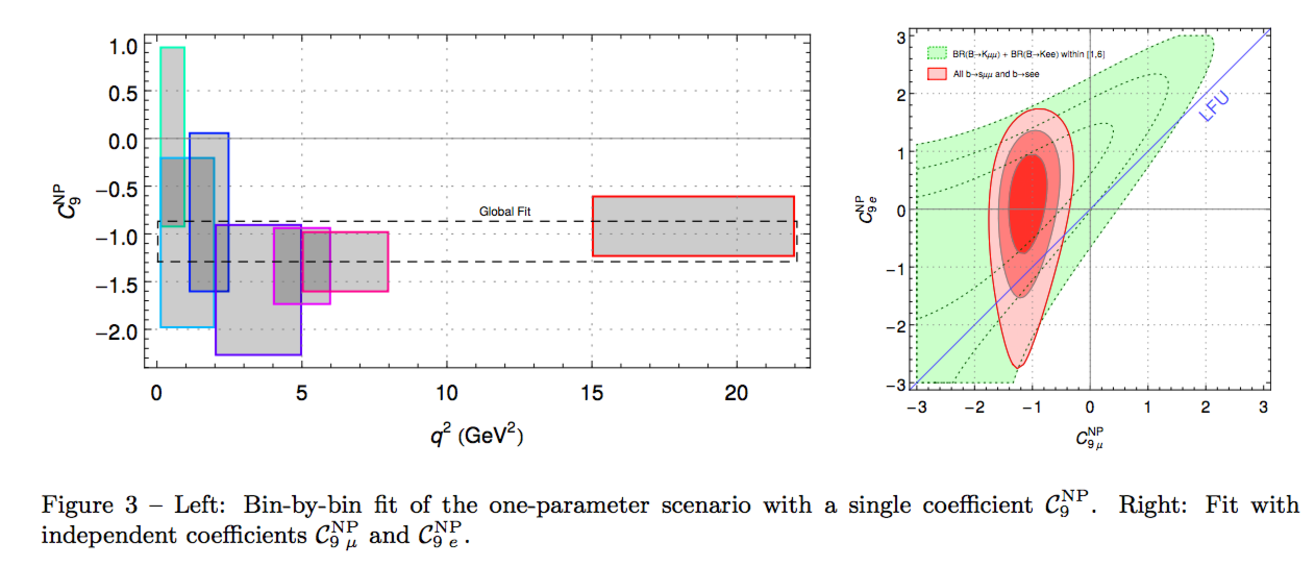
\includegraphics[width=15cm]{rare_fit.pdf}
\end{center}
\caption{Phenomenological analysis of the rare decays constraints on NP from~\cite{Descotes-Genon:2016hem}. The left plot shows the global fit results of the Wilson coefficients when only the new physics coefficient $C_9^{NP}$, currently exhibiting the largest deviation from 0,  is left floating. The fit is performed in  different bins of $q^2$. The right plot shows the constraints in the hypothesis of independent electron and muon coefficients $C_{9e}^{NP}$ and  $C_{9\mu}^{NP}$, which is a test of lepton flavor universality.}%
\label{figrare}%
\end{figure}




\subsection*{Plans for the GDR}
 Following and improving  the good experience of the PEPS-PTI projects on rare decays, the following topics would be addresses in the context of  the GDR with a strict collaboration between theorists and experimentalists.
\begin{itemize}
\item For the angular analyses of $b \to sll$ transitions, with the new and more accurate experimental data, it becomes mandatory to assess the hadronic uncertainties on the theory side. Lattice QCD and the QCD sum rule practitioners will try and 
evaluate the size of theoretical errors and discuss the appropriate methodology on how to account for various sources of systematic uncertainties. We should explore the  $B^0\to K^\ast \tau\tau$ channel and define new observables taking into account the direct access to the $\tau$ polarization. The study of $b \to s \ell \ell$ transition in $b$-baryons  is quite new and the identification of interesting observables for the $\Lambda_b \to \Lambda^\ast \mu\mu$ decay may be interesting.  
Possible phenomenological ideas on how to relate the hadronic quantities in several decay modes will be discussed, as they might be helpful in canceling a large part of hadronic uncertainties.
Ideas on how to treat the non-resonant $c\bar c$-contributions would be very welcome. The phenomenological interpretation of the experimental results will allow to shed lights on which physics beyond SM best fits the data. 
\item For the photon polarization measurements, the $B^0\to K^\ast e e $ will benefit of the additional statistics collected already by the Run2 of LHCb. In addition,  direct measurements of the photon polarisation in  the radiative decays 
$B0 \to f_{CP}\gamma$ and $B \to(hhh)\gamma$ modes (here $h$ is a kaon or a pion) will be pursued, with a detailed study of the resonant structure of the decay. The complementarity and interplay with the measurements at Belle II will be addressed. It will be worth also to explore the possibility of observing the suppressed $b\to d\gamma$ transitions and search for $B_s\to \gamma \gamma$ decays. 
\item Concerning the LFUV, we should elaborate a general scenario of NP, in an effective field theory approach, allowing to isolate the  observables  which are most sensitive to the couplings to the vector (scalar) and/or axial (pseudoscalar) operators. Experimenters and theorists will elaborate on the feasibility of the distribution of $B_{(s)}\to D_{(s)}^\ast  \ell \nu_\ell$ decays according to the polarization of the outgoing vector meson. Furthermore, a contact with other leptonic observables should be made in order to test several plausible scenarios of NP which result in LFUV. New experimental results on the ratio measurements will be provided by LHCb, with a direct involvement of the French groups, but are also expected from Belle II. 
\item The LFV direct searches will soon provide new results, both in LHCb and later in Belle II, as well as in dedicated experiments (COMET, MEG, Mu2e, Mu3e). It will be crucial to work on a package that could include all the possible constraints relevant to LFV at low and high energy and see what are the lessons one can learn about the Yukawa sector from the data. The interplay with the lepton sector here is crucial, and will be addressed  with more details in section~\ref{sec:lepfla}. 
\item Finally we should assess the current situation concerning the extraction of the Yukawa couplings from experimental data, clarifying in which way those data can be related to the low-energy physics observables and 
$b$-decay observables in particular. In order to address the issue "{\it Which theory of flavor?}",  we will try and combine the searches made at Belle~II with those made at NA62 and KOTO experiments.  
We should also address the issue of the (in)compatibility of the conclusions found in the Yukawa sector through the low-energy experiments with the LHC findings at the TeV-scale. 
\end{itemize} 

%
%
%\begin{figure}[!htb]
%\begin{center}
%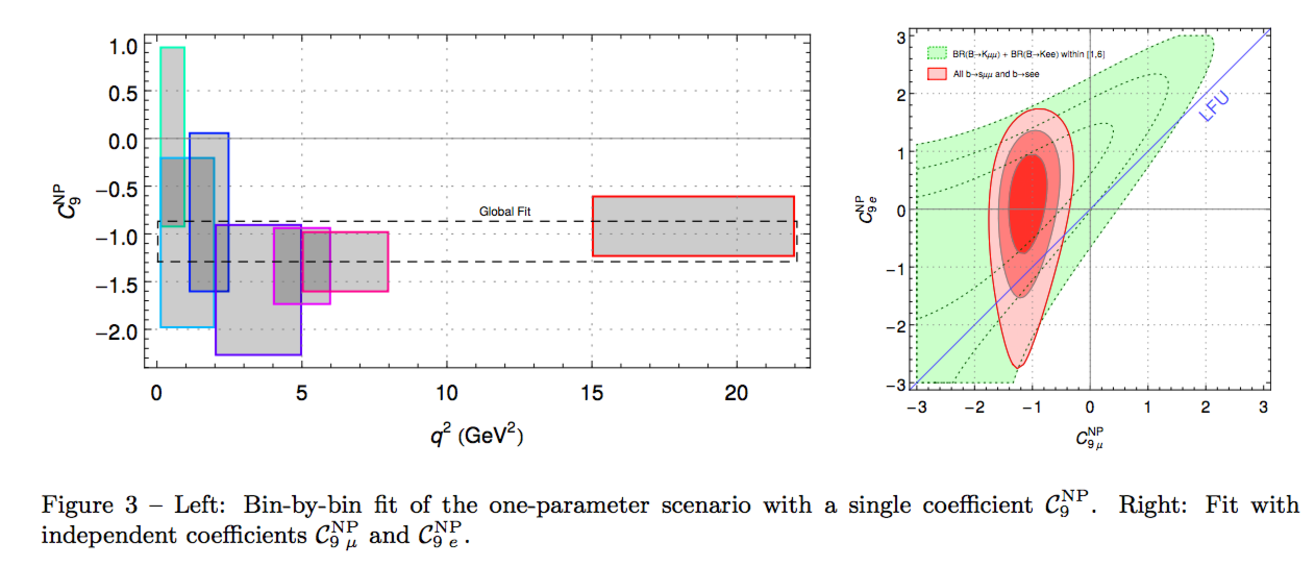
\includegraphics[width=14cm]{rare_fit.pdf}
%\end{center}
%\caption{ From arXiv:1605.06059v1 \bf{will develop the caption}}%
%\label{figphis}%
%\end{figure}
%


%%A proposed timeline for the annual workshops is described below. 
%\begin{enumerate}
%\item Year One: Workshop on the LFUV in $B$ and $B_s$ decays\\ 
%During this workshop the theorists will discuss a general scenario of NP, in an effective field theory approach, and isolate the observables which are most sensitive 
%to the couplings to the vector (scalar) and/or axial (pseudoscalar) operators. Experimenters and theorists will elaborate on the feasibility of the distribution of $B_{(s)}\to D_{(s)}^\ast  \ell \nu_\ell$ 
%according to the polarization of the outgoing vector meson. Furthermore, a contact with other leptonic observables should be made in order to test several plausible scenarios of NP which 
%result in LFUV.
%
%\vskip .6cm 
%
%\item Year Two: Workshop on the angular distribution of various decay modes\\ 
%With the new and more accurate experimental data it becomes mandatory to assess the hadronic uncertainties on the theory side. Lattice QCD and the QCD sum rule practitioners will try and 
%evaluate the size of theoretical errors and discuss the appropriate methodology on how to account for various sources of systematic uncertainties. 
%Another interesting subject could be the angular analysis of $B^0\to K^\ast \tau\tau$ and the study of new observables taking into account the direct access to the $tau$ polarization.
%The study of $b \to s \ell \ell$ transition in b-baryons  is quite new and the identification of interesting observables for the $\Lambda_b \to \Lambda^\ast \mu\mu$ may be interesting.  
%Possible phenomenological ideas on how to relate the hadronic quantities in several decay modes will be discussed as they might be helpful in cancelling a large part of hadronic uncertainties.
%Ideas on how to treat the non-resonant $c\bar c$-contributions would be very welcome. Participants will also address the question {\it ``Which physics BSM?"}
%
%\vskip .6cm 
%
%\item Year Three: Workshop on the lepton flavor violation in $b$-decays\\ 
%Revisiting the LFUV problem: discuss the new constraints on  $R_{K^{(\ast )}, D^{(\ast )}, \Lambda^{(\ast )}}$ obtained in Belle~II, and attempt drawing more accurate conclusions concerning the 
%new physics scenarios. Focus then on the LFV modes and on interpretation of the results found by LHCb. The issues related to the identification of $\tau$ in the final state should be revisited. 
%Work on the package of codes that would include all possible constraints relevant to the LFV at low and high energy and see what are the lessons one can learn about the Yukawa sector from the data. 
%
%\vskip .6cm 
%
%\item Year Four: Workshop on the relation to Higgs \\ 
%Assess the current situation concerning the extraction of the Yukawa couplings from experimental data. In what way those data can be related to the low-energy physics observables and 
%$b$-decay observables in particular. In order to address the issue of ``{\it Which theory of flavor?}" we will try and combine the searches made at Belle~II with those made at NA62 and KOTO experiments. 
%Address the issue of (in)compatibility of the conclusions found in the Yukawa sector through the low-energy experiments with the LHC findings at the TeV-scale. 
%
%\end{enumerate}
